% Options for packages loaded elsewhere
\PassOptionsToPackage{unicode,linktoc=all}{hyperref}
\PassOptionsToPackage{hyphens}{url}
\PassOptionsToPackage{dvipsnames,svgnames,x11names}{xcolor}
%
\documentclass[
  a4paper,
]{article}
\usepackage{amsmath,amssymb}
\usepackage{iftex}
\ifPDFTeX
  \usepackage[T1]{fontenc}
  \usepackage[utf8]{inputenc}
  \usepackage{textcomp} % provide euro and other symbols
\else % if luatex or xetex
  \usepackage{unicode-math} % this also loads fontspec
  \defaultfontfeatures{Scale=MatchLowercase}
  \defaultfontfeatures[\rmfamily]{Ligatures=TeX,Scale=1}
\fi
\usepackage{lmodern}
\ifPDFTeX\else
  % xetex/luatex font selection
\fi
% Use upquote if available, for straight quotes in verbatim environments
\IfFileExists{upquote.sty}{\usepackage{upquote}}{}
\IfFileExists{microtype.sty}{% use microtype if available
  \usepackage[]{microtype}
  \UseMicrotypeSet[protrusion]{basicmath} % disable protrusion for tt fonts
}{}
\makeatletter
\@ifundefined{KOMAClassName}{% if non-KOMA class
  \IfFileExists{parskip.sty}{%
    \usepackage{parskip}
  }{% else
    \setlength{\parindent}{0pt}
    \setlength{\parskip}{6pt plus 2pt minus 1pt}}
}{% if KOMA class
  \KOMAoptions{parskip=half}}
\makeatother
\usepackage{xcolor}
\usepackage[margin=25mm]{geometry}
\usepackage{longtable,booktabs,array}
\usepackage{calc} % for calculating minipage widths
% Correct order of tables after \paragraph or \subparagraph
\usepackage{etoolbox}
\makeatletter
\patchcmd\longtable{\par}{\if@noskipsec\mbox{}\fi\par}{}{}
\makeatother
% Allow footnotes in longtable head/foot
\IfFileExists{footnotehyper.sty}{\usepackage{footnotehyper}}{\usepackage{footnote}}
\makesavenoteenv{longtable}
\usepackage{graphicx}
\makeatletter
\def\maxwidth{\ifdim\Gin@nat@width>\linewidth\linewidth\else\Gin@nat@width\fi}
\def\maxheight{\ifdim\Gin@nat@height>\textheight\textheight\else\Gin@nat@height\fi}
\makeatother
% Scale images if necessary, so that they will not overflow the page
% margins by default, and it is still possible to overwrite the defaults
% using explicit options in \includegraphics[width, height, ...]{}
\setkeys{Gin}{width=\maxwidth,height=\maxheight,keepaspectratio}
% Set default figure placement to htbp
\makeatletter
\def\fps@figure{htbp}
\makeatother
\setlength{\emergencystretch}{3em} % prevent overfull lines
\providecommand{\tightlist}{%
  \setlength{\itemsep}{0pt}\setlength{\parskip}{0pt}}
\setcounter{secnumdepth}{-\maxdimen} % remove section numbering
\newlength{\cslhangindent}
\setlength{\cslhangindent}{1.5em}
\newlength{\csllabelwidth}
\setlength{\csllabelwidth}{3em}
\newlength{\cslentryspacingunit} % times entry-spacing
\setlength{\cslentryspacingunit}{\parskip}
\newenvironment{CSLReferences}[2] % #1 hanging-ident, #2 entry spacing
 {% don't indent paragraphs
  \setlength{\parindent}{0pt}
  % turn on hanging indent if param 1 is 1
  \ifodd #1
  \let\oldpar\par
  \def\par{\hangindent=\cslhangindent\oldpar}
  \fi
  % set entry spacing
  \setlength{\parskip}{#2\cslentryspacingunit}
 }%
 {}
\usepackage{calc}
\newcommand{\CSLBlock}[1]{#1\hfill\break}
\newcommand{\CSLLeftMargin}[1]{\parbox[t]{\csllabelwidth}{#1}}
\newcommand{\CSLRightInline}[1]{\parbox[t]{\linewidth - \csllabelwidth}{#1}\break}
\newcommand{\CSLIndent}[1]{\hspace{\cslhangindent}#1}
\ifLuaTeX
\usepackage[bidi=basic]{babel}
\else
\usepackage[bidi=default]{babel}
\fi
\babelprovide[main,import]{british}
% get rid of language-specific shorthands (see #6817):
\let\LanguageShortHands\languageshorthands
\def\languageshorthands#1{}
% $HOME/.pandoc/defaults/latex-header-includes.tex
% Common header includes for both lualatex and xelatex engines.
%
% Preliminaries
%
% \PassOptionsToPackage{rgb,dvipsnames,svgnames}{xcolor}
% \PassOptionsToPackage{main=british}{babel}
\PassOptionsToPackage{english}{selnolig}
\AtBeginEnvironment{quote}{\small}
\AtBeginEnvironment{quotation}{\small}
\AtBeginEnvironment{longtable}{\centering}
%
% Packages that are useful to include
%
\usepackage{graphicx}
\usepackage{subcaption}
\usepackage[inkscapeversion=1]{svg}
\usepackage[defaultlines=4,all]{nowidow}
\usepackage{etoolbox}
\usepackage{fontsize}
\usepackage{newunicodechar}
\usepackage{pdflscape}
\usepackage{fnpct}
\usepackage{parskip}
  \setlength{\parindent}{0pt}
\usepackage[style=american]{csquotes}
% \usepackage{setspace} Use the <fontname-plus.tex> files for setspace
%
\usepackage{hyperref} % cleveref must come AFTER hyperref
\usepackage[capitalize,noabbrev]{cleveref} % Must come after hyperref
% noto-plus.tex
% Font-setting header file for use with Pandoc Markdown
% to generate PDF via LuaLaTeX.
% The main font is Noto Serif.
% Other main fonts are also available in appropriately named file.
\usepackage{fontspec}
\usepackage{setspace}
\setstretch{1.3}
%
\defaultfontfeatures{Ligatures=TeX,Scale=MatchLowercase,Renderer=Node} % at the start always
%
% For English
% See also https://tex.stackexchange.com/questions/574047/lualatex-amsthm-polyglossia-charissil-error
% We use Node as Renderer for the Latin Font and Greek Font and HarfBuzz as renderer ofr Indic fonts.
%
\babelfont{rm}[Script=Latin,Scale=1]{NotoSerif}% Config is at $HOME/texmf/tex/latex/NotoSerif.fontspec
\babelfont{sf}[Script=Latin]{SourceSansPro}% Config is at $HOME/texmf/tex/latex/SourceSansPro.fontspec
\babelfont{tt}[Script=Latin]{FiraMono}% Config is at $HOME/texmf/tex/latex/FiraMono.fontspec
%
% Sanskrit, Tamil, and Greek fonts
%
\babelprovide[import, onchar=ids fonts]{sanskrit}
\babelprovide[import, onchar=ids fonts]{tamil}
\babelprovide[import, onchar=ids fonts]{greek}
%
\babelfont[sanskrit]{rm}[Scale=1.1,Renderer=HarfBuzz,Script=Devanagari]{NotoSerifDevanagari}
\babelfont[sanskrit]{sf}[Scale=1.1,Renderer=HarfBuzz,Script=Devanagari]{NotoSansDevanagari}
\babelfont[tamil]{rm}[Renderer=HarfBuzz,Script=Tamil]{NotoSerifTamil}
\babelfont[tamil]{sf}[Renderer=HarfBuzz,Script=Tamil]{NotoSansTamil}
\babelfont[greek]{rm}[Script=Greek]{GentiumBookPlus}
%
% Math font
%
\usepackage{unicode-math} % seems not to hurt % fallabck
\setmathfont[bold-style=TeX]{STIX Two Math}
\usepackage{amsmath}
\usepackage{esdiff} % for derivative symbols
%
%
% Other fonts
%
\newfontfamily{\emojifont}{Symbola}
%

\usepackage{titling}
\usepackage{fancyhdr}
    \pagestyle{fancy}
    \fancyhead{}
    \fancyfoot{}
    \renewcommand{\headrulewidth}{0.2pt}
    \renewcommand{\footrulewidth}{0.2pt}
    \fancyhead[LO,RE]{\scshape\thetitle}
    \fancyfoot[CO,CE]{\footnotesize Copyright © 2006\textendash\the\year, R (Chandra) Chandrasekhar}
    \fancyfoot[RE,RO]{\thepage}
\newfontfamily{\regulariconfont}{Font Awesome 6 Free Regular}[Color=Grey]
\newfontfamily{\solidiconfont}{Font Awesome 6 Free Solid}[Color=Grey]
\newfontfamily{\brandsiconfont}{Font Awesome 6 Brands}[Color=Grey]
%
% Direct input of Unicode code points
%
\newcommand{\faEnvelope}{\regulariconfont\ ^^^^f0e0\normalfont}
\newcommand{\faMobile}{\solidiconfont\ ^^^^f3cd\normalfont}
\newcommand{\faLinkedin}{\brandsiconfont\ ^^^^f0e1\normalfont}
\newcommand{\faGithub}{\brandsiconfont\ ^^^^f09b\normalfont}
\newcommand{\faAtom}{\solidiconfont\ ^^^^f5d2\normalfont}
\newcommand{\faPaperPlaneRegular}{\regulariconfont\ ^^^^f1d8\normalfont}
\newcommand{\faPaperPlaneSolid}{\solidiconfont\ ^^^^f1d8\normalfont}

%
% The block below is commented out because of Tofu glyphs in HTML
%
% \newcommand{\faEnvelope}{\regulariconfont\ \normalfont}
% \newcommand{\faMobile}{\solidiconfont\ \normalfont}
% \newcommand{\faLinkedin}{\brandsiconfont\ \normalfont}
% \newcommand{\faGithub}{\brandsiconfont\ \normalfont}
\ifLuaTeX
  \usepackage{selnolig}  % disable illegal ligatures
\fi
\IfFileExists{bookmark.sty}{\usepackage{bookmark}}{\usepackage{hyperref}}
\IfFileExists{xurl.sty}{\usepackage{xurl}}{} % add URL line breaks if available
\urlstyle{sf}
\hypersetup{
  pdftitle={The Most Scary Experience},
  pdfauthor={R (Chandra) Chandrasekhar},
  pdflang={en-GB},
  colorlinks=true,
  linkcolor={DarkOliveGreen},
  filecolor={Purple},
  citecolor={DarkKhaki},
  urlcolor={Maroon},
  pdfcreator={LaTeX via pandoc}}

\title{The Most Scary Experience}
\author{R (Chandra) Chandrasekhar}
\date{2023-07-14 | 2023-11-27}

\begin{document}
\maketitle

\thispagestyle{empty}


\hypertarget{probing-fear}{%
\subsection{Probing fear}\label{probing-fear}}

My \href{https://www.thefreedictionary.com/redoubtable}{redoubtable}
friend Solus ``Sol'' Simkin wandered into my office late one afternoon
and asked me, ``What is the most scary experience for a human being?''

I thought but for an instant as I replied, almost reflexively, ``Death.
What else? Or a close shave with death.''

The hard taskmaster that he is, Sol told me to think again. He told me
to imagine a fear that will not disappear, but like a shadow,
relentlessly pursues one's days and nights. A fear with no respite. Not
the fear of encountering a cobra, or a black mamba, that wears off in
half an hour at most. Not the fear of a narrowly missed road accident
that leaves one rattled and shivering for a full five minutes. Not the
transient thrill of the roller-coaster. Nor the fear of falling. No,
this is a shoreless fear. And nothing supernatural. It is a fear as
mundane as the Earth and yet, it is a fear that we do not normally
encounter, let alone experience. But when recognized and felt, it is a
fear that chills the spine and shakes one's very core.

``Sol,'' I said. What you are asking me to probe calls for long, deep,
and hard thought. I need more time, for sure.''

\hypertarget{homework}{%
\subsection{Homework}\label{homework}}

``Take your time, and wend your way slowly through the labyrinth of your
own memories and pluck for me that single, shiny nugget of fear that
dazzles you even today---its power to enchant, enthrall, and engulf,
undiminished by the passage of time,'' Sol told me soothingly. ``I have
a reason for asking you to undertake this introspection. I had my own
close brush with depthless fear recently. What I learned from it was
unusual, to say the least. I wish to discuss it with you after you have
done your own inner exploration. So, when you are ready, we will discuss
it in the relaxing and reassuring confines of our favourite coffeehouse.
Mind you, be prepared for many sessions before the
\href{https://www.thefreedictionary.com/denouement}{denouement} takes
place!''

\hypertarget{the-genre-of-horror-fiction}{%
\subsection{The genre of horror
fiction}\label{the-genre-of-horror-fiction}}

Vicarious experiences are always easier to draw upon, and for the
category of fear, there is the ready-made genre of horror fiction.
Before my next meeting with Sol, I tried to assemble a quick list of
scary tales from
\href{https://americanliterature.com/author/hh-munro-saki}{H H Munro's}
\href{https://www.classicshorts.com/stories/vashtar.html}{\emph{Shredni
Vashtar}}, to \href{https://www.hplovecraft.com/}{H P Lovecraft's}
\href{https://www.hplovecraft.com/writings/texts/fiction/cc.aspx}{\emph{The
Call of Cthulhu}}. Then there was
\href{https://openlibrary.org/books/OL4122966M/The_Arbor_House_treasury_of_horror_and_the_supernatural}{\emph{The
Arbor House Treasury of Horror and the Supernatural}} which had
engrossed me for many days and nights with its eclectic collection of
terrifying tales, but none of them had left me a hapless heap of jelly,
paralyzed with fear.

Then I remembered one of my favourite authors,
\href{https://www.poetryfoundation.org/poets/edgar-allan-poe}{Edgar
Allan Poe}, and his
\href{https://www.amazon.in/Tales-Mystery-Imagination-Collins-Classics/dp/0007420226}{\emph{Tales
of Mystery and Imagination}}, surely among the choicest morsels of the
macabre. The injection of fear from these stories had been swift and
intense, but not long-lasting. Even the movie,
\href{https://www.imdb.com/title/tt0081505/}{\emph{The Shining}}, based
on angst-meister
\href{https://www.britannica.com/biography/Stephen-King}{Stephen King's}
novel of the same name, had been able to terrify me, but only
fleetingly.

I came to the conclusion that, no matter how good, ideas imposed from
the outside, as in short stories or movies, did not possess the power to
frighten as intensely one's own inner experiences. A dream, spun from
the yarn of a short story, and convoluted to one's fancy, is more potent
in invoking fear than the original short story itself. \emph{Personal
input is a necessary ingredient for gut-wrenching terror}.

When I met Sol a week later, I shared this insight with him. He nodded
in agreement and told me to continue.

I said that the \emph{unexpected} in any situation stimulated fear as we
were wired to the
\href{https://www.verywellmind.com/what-is-the-fight-or-flight-response-2795194}{fight
or flight} response to ensure survival. The hormones released in the
process give fear its physical manifestations. Fact or fiction, however
well crafted, could not match the immediacy of a physical threat to
induce acute but short-lived fear.

The \href{http://www.orchardvalleycoffee.net/}{Orchard Valley Coffee
House} was our cosy haven for kaffeeklatsch, where we explored at
leisure the twists and turns of fear. We stayed quiet awhile, gently
sipping a latte and nibbling at a cherry cake. After a little discussion
and an eloquent silence, we agreed to meet again. Sol said, ``We have
but scratched the surface. The immensity of the iceberg of fear is
largely hidden. Let us meet again to chat. I find our exchanges
insightful.''

\hypertarget{juvenile-tales}{%
\subsection{Juvenile tales}\label{juvenile-tales}}

After my foray into the literature of horror and terror, I decided to
review the fondly remembered stories of early childhood, in case they
held the key to the most scary experience. Was there anything in the
corpus of juvenile literature that evoked the bogeyman? Had I ever been
terrified by a tale from my past?

As I mulled over the stories of my childhood, I realized that, save for
a dozen or so tales, most were misty recollections that became amorphous
when pursued. So, I tried to remember the memorable stories--- those
that remained with me decades after I had read them, because they
illumined some aspect of life with a golden glow. But could the warmth
of fond memories unearth the fear of the century?

I fell into a short but vivid reverie, or was it what in German is
called
\href{https://de.pons.com/\%C3\%BCbersetzung/deutsch-englisch/Halbschlaf}{\emph{Halbschlaf}}---that
delicious state between wakefulness and sleep, that hypnagogic heaven,
where reality and dreams are fused indistinguishably. When I woke up
again after a half hour, I felt that I had ridden a camel in the searing
Arabian desert, and later enjoyed the hospitality of the
\href{https://www.newworldencyclopedia.org/entry/Bedouin}{Bedouin}.

I racked my brain trying to remember a book from my childhood, about
camels and the Bedoiun, that held some truth about fear. No, most
juvenile books are written, not to stoke fear but to spread cheer. Was
it the famed
\href{https://www.newworldencyclopedia.org/entry/The_Book_of_One_Thousand_and_One_Nights}{\emph{Tales
of a Thousand Nights and One Night}}? While entertaining stratagems,
nail-biting adventures, and twists and turns of plot abounded in that
beloved childhood book, nothing so dark as irredeemable fear ever
stalked its pages.

\hypertarget{the-miracle-of-hope}{%
\subsection{The miracle of hope}\label{the-miracle-of-hope}}

A few days later, I heard the unspoken word `hope' insistently
clamouring for my attention. Thinking that `hope' might become
``hopeless'' in my quest for the most scary experience, I diverted
myself to other, more pressing matters. The drumbeat `hope' became the
silent heartthrob `hope' in my inner ear. But it refused to go away, try
what I might.

After three days of `hope', I remembered in a flash a gentle story of my
\href{https://www.thefreedictionary.com/tween}{tween} years. I had
borrowed a book from the local library and it was about a camel. That
library was long gone and the best I could do to recollect the name of
the book was to search the Web. The book, long out-of-print, was still
incarnate in digital form at the archive named after
\href{https://www.newworldencyclopedia.org/entry/Johannes_Gutenberg}{Gutenberg},
God bless his soul! {[}\protect\hyperlink{ref-boyle1939}{1}{]}

It was called \emph{The Youngest Camel} and was written by Kay Boyle,
illustrated by Fritz Kredel, and published in 1939 by `Little, Brown,
and Company'. Its digital reincarnation happened in 2021 as
\href{https://www.gutenberg.org/files/64988/64988-h/64988-h.htm}{eBook
\#64988}. As I gazed upon the book cover, shown in \cref{fig:camel}, I
could almost feel the ribbed texture of the fabric cover against my
fingers, after all these years.

\begin{figure}
\hypertarget{fig:camel}{%
\centering
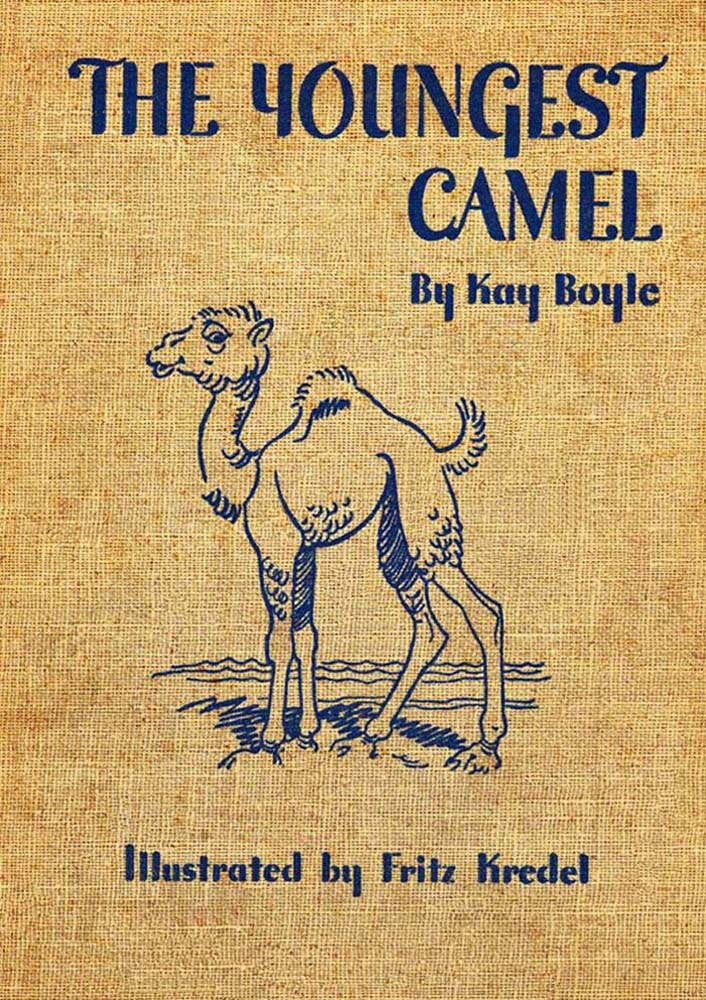
\includegraphics[width=0.4\textwidth,height=\textheight]{images/camel.jpg}
\caption{The book cover of \emph{The Youngest Camel}.}\label{fig:camel}
}
\end{figure}

But what did this treasure from my childhood have to do with `hope'? The
digital age has its uncontested benefits, and one of them is the
possibility of \emph{digital search}. Instead of scanning through a
thick wad of printed pages, all one needed to do was to type in the
keyword being searched for, and voila, one had a half-dozen matches or
so. That is exactly what I did with the \emph{The Youngest Camel}. After
a few hops and skips, there it was:

\begin{quote}
``Why is the word `hope' magic?'' asked the youngest camel, stretching
out one stiff leg to see if it still could move. And now Mohammed's son
lifted the little camel's head up again and laid it against his shoulder
while he shook the remaining cords away. When he did this, the little
camel saw that he was young and very handsome. He was wearing a silk
turban with pearls and turquoises embroidered on it, and carved gold
ornaments hung from his ears, and there was a look of great gentleness
in his face.
\end{quote}

\begin{quote}
``Well, you see, h stands for `help,' and o stands for `O,' and p stands
for `power,' and e stands for `eternal,'\,'' he said so lightly and
merrily that he seemed to be making fun of something. He took out a
little ivory flask from his garments and poured some fresh water between
the little camel's burning lips. ``So when you say `hope' like that,
you're really saying `Help, O power eternal!' And that means me because
I've been appointed your patron saint this year.''
\end{quote}

\begin{center}

\textbf{H}elp\\
\textbf{O}\\
\textbf{P}ower\\
\textbf{E}ternal!

\end{center}

And there it was. Hope is actually a prayer that connects us with the
Eternal Power. And people devoid of hope are literally \emph{hopeless}.
They do not live; they just waste away. That was the message from the
book of my childhood to my adult self.

\hypertarget{hopelessness-and-pows}{%
\subsection{Hopelessness and POWs}\label{hopelessness-and-pows}}

That brought to mind a poignant article that I had chanced upon one day,
entitled, ``The Prison of Hopelessness'' by an American Air Force
Chaplain {[}\protect\hyperlink{ref-wilson2006}{2}{]}. It was a sobering,
thought-provoking article. While we all need food, water, sunshine, and
clean air to be healthy, the emotions that populate our minutes and days
are equally potent factors affecting our well-being. A quick web search
informed me that the unholy triad of helplessness, hopelessness, and
worthlessness were potent factors leading to depression and death.

``There you have it!'' I thought triumphantly. I had the answer that
would clinch success at my next meeting with Sol. The most scary
experience in the world is hopelessness: it disconnects us from our
Source and feeds helplessness and worthlessness, leading to gloom, doom,
and tragedy. From the sunny story of \emph{The Youngest Camel} to the
dark depths of depression, it was hope that lit the way, and its absence
that fed fear and pessimism.

\hypertarget{with-sol-again}{%
\subsection{With Sol again}\label{with-sol-again}}

At my next meeting with Sol, I poured out my newfound knowledge with the
panache of an honours student defending his thesis. Sol flattered me
with unwavering attention, assimilating all I said, amidst sips of the
finest of lattes.

After a thoughtful pause, he said, ``What you have stumbled upon in a
convoluted fashion is indeed the cause of deep and searing wounds on the
human psyche. Enough sometimes, to persuade a person to `give it all
up.' But notice one thing. It is the result of \emph{external}
circumstances impinging on the self that leads to this. Wouldn't
something nearer the self be even more horrific. Could you take a
guess?''

``Loneliness, or grief, or the loss of a loved one. Something serious
like that,'' I ventured.

``Even that comes from the outside,'' he said. And I nodded in
agreement.

The gravity of the subject was an ample excuse for an extra mocha latte
and some special cakes to lift our spirits. Having spent a good two
hours exchanging rarefied philosophical thoughts we bid each other
\emph{au revoir}.

\hypertarget{the-void}{%
\subsection{The Void}\label{the-void}}

When the Lord Buddha sat under the tree, pondering life's sorrows and
their causes, he identified desire as the chieftain of all miseries. But
the solution he gave was an even more scary proposition. The Void.
Imagine being swallowed into the Void. Losing all sense of self and not
knowing whether one would continue to exist thereafter or not.

I thought of my own experience at a swimming pool late one night. It was
half an hour from closing time when I started my swim. The floodlights
and the water ripples were projecting undulating patterns of light on
the pool bottom, called \emph{caustics}, shown in
\cref{fig:water-caustic}. There were still a good ten swimmers in the
pool. As the minutes ticked away, they left one by one, until I was
alone in the pool, when the whistle was blown to notify us that the
swimming pool would be closing in ten minutes.

\begin{figure}
\hypertarget{fig:water-caustic}{%
\centering

\includegraphics[width=0.75\textwidth,height=\textheight]{images/water-caustic.jpg}
\caption[Picture of water caustics at the bottom of a swimming
pool.]{Picture of water caustics at the bottom of a swimming
pool.\footnotemark{}}\label{fig:water-caustic}
}
\end{figure}
\footnotetext{Image courtesy of Ha4ipuri. Original is
  \href{https://photodune.net/item/blue-swimming-pool-underwater-with-bright-sun-light-reflections-or-caustics-background-or-texture/46148405}{here}.}

It was comforting to be in the pool when others were also swimming
because they churned the water enough to make those mesmerizing ripples
of light on the pool floor. But when I was swimming solo in the pool, I
felt a cold wave of fear. The friendly ubiquitous patterns of light had
disappeared, leaving me only with my self-made ripples.

I thought of each swimmer metaphorically as a thought, and when I was
alone in the pool, I represented the last thought. The extinguishing of
that last thought in \_nirvana\_or \emph{samadhi} would be a fearful
experience because it would shake the very foundations of the self we
are. We would be swallowed up by the immensity of the Void, or the pool
in this case.

I determined that I would bring up the Void when I next met Sol to
resume our discussion on the most scary experience.

\hypertarget{the-most-scary-experience}{%
\subsection{The most scary experience}\label{the-most-scary-experience}}

Our next meeting at our favourite haunt was on a public holiday, and
started at the mellow hour of ten in the morning. Eagerly, I told Sol
that I had cracked his conundrum. The fear of being swallowed by the
Void was clearly the most scary experience. I then narrated my own
episode at the swimming pool.

He listened with rapt attention and then asked me penetratingly, ``Did
you survive the experience?''

I answered that obviously I had, adding that I was forced to get out of
the pool anyway by the ``time's up'' whistle.

``Were you so scared that you had to be helped out of the pool?''

``No,'' I answered truthfully. ``I got out without difficulty, but was a
little unnerved. That is all.''

``Would you go into a pool to swim again after this?''

``Of course!'' I said. ``I count swimming among life's premium
pleasures. It helps me de-stress and relax. It helps my thoughts to flow
as freely as the water. Indeed, I have solved many a knotty problem in
the pool. And, what's more, it is a healthy exercise.''

``And you want me to take your single episode in the pool and admit it
as life's most scary experience? Surely, you are joking,'' Sol added
ironically.

Looking outside the coffee house at the warmth of the full morning sun,
and the gentle ripple of leaves in the wind, I felt a little sheepish.
``Well, I thought that fear of the Void was an ace candidate: a finalist
at the very least!'' I said appealingly.

``That I grant you,'' said Sol. It was so difficult to get the least
approbation from him that I felt grateful for his remark. ``Fear of loss
of one's identity is indeed among the great fears that assail humankind.
That is why people fear death. They do not know whether their identity
will survive the experience.

``But if the reports from countless
\href{https://en.wikipedia.org/wiki/Near-death_experience}{NDEs (Near
Death Experiences)} are to be believed, death is a transition from one
state of consciousness to another, and has nothing to do with loss of
identity, any more than waking up from a dream does. Just as a dream is
dissolved upon waking up, so does the `dream of this world' get
dissolved when we die, to wake up in another state of consciousness. But
loss of identity, there isn't.''

``OK, Sol,'' I said. ``I have exhausted myself pondering the question
you set me weeks ago. Why don't we call it a draw, and you tell me the
answer. My idea of the Void has at least found honourable mention, I
believe.''

Sol smiled wryly and said, ``It is such a fine day, bright and carefree.
Let us take a walk outdoors, commune with Mother Nature, and enjoy the
weather. There will always be other days, grey and overcast, that will
be more in tune with the topic we are discussing.''

And so we left abruptly to enjoy the sunny outdoors.

\hypertarget{the-denouement}{%
\subsection{The denouement}\label{the-denouement}}

The Saturday next week was cold and gloomy---a perfect backdrop to a
discussion of the most scary experience. I met Sol at our cafe and each
of us ordered his favourite coffee brew and choice of cake. We continued
where we left off.

Sol began, saying, ``Did I ever tell you how I felt about finishing my
PhD? Every day for six years, the PhD was all I could think of. It
weighed on me like a slab that couldn't be dislodged, until that happy
day when I handed in my thesis.''

``When I woke up the next morning,'' he continued, ``I missed the
slab---the weight of the unfinished thesis. I told myself that I should
be euphoric for I had at last been let out of the self-imposed PhD
prison. But I really missed having an unfinished thesis. I think it was
a bit like the
\href{https://en.wikipedia.org/wiki/Stockholm_syndrome}{Stockholm
syndrome}, or the
\href{https://www.mayoclinic.org/diseases-conditions/postpartum-depression/symptoms-causes/syc-20376617}{postpartum
baby blues} suffered by a young mother who has just given birth to her
first child. Even
\href{https://www.health.harvard.edu/mens-health/retirement-stress-taking-it-too-easy-can-be-bad-for-you}{retirement
can be stressful}. We fall in love with our trials.''

``And did you get over it?'' I asked.

``I got used to it,'' he said. ``Like the mist that lifts gradually with
the morning sun, I became gradually accustomed to life without the
burden of a PhD thesis. And after a while, I did not miss it any more.
Out of sight, out of mind.''

``So what is your definitive take on the most scary experience---more
scary than everything we have discussed so far? And we have covered
quite a bit,'' I said.

He looked at me wistfully and then turned his gaze to the large glass
windows in the cafe, staring vacantly into the outside, before resuming
our conversation. With unaccustomed humility, he said ``I am in no way
superior to anyone else that my pronouncement should be deemed final in
this `most scary experience' competition. But what I am about to tell
you is my personal experience.''

``Imagine that you lose something like your sense of identity but you
are still living. The fear of loss of identity, with death or with
enlightenment, is perhaps something neither of us will encounter in the
here and now. But what happens if you went through a thorough clearing
out of your `To Do' tray in life. I had a foretaste of that after I
submitted my PhD thesis, but it was temporary. \emph{But what happens
when you really feel that there is nothing else for you to accomplish in
this world?}''

I was taken aback by the utter finality of what he said. ``Did some
event in your life trigger such a feeling?'' I asked.

``Let me explain the context,'' he said after a few moments. ``It was a
good six months ago. I was laid up in bed for eight days with influenza.
I was isolated in my room so as not to spread the virus to others. Those
eight days were restful but when I recall them now, they feel like a
blur. I cannot recall individual days or daily experiences. But on the
day I became well enough to leave my isolation, I got up from bed and
felt that I had \emph{nothing more to accomplish in the world}. It was
not a result of thought but what I may call \emph{pure knowing}.''

``So, it was a more extreme form of your PhD-thesis-withdrawal
syndrome?'' I asked.

Sol nodded. ``What was strange was that this `no unfinished business'
feeling was not triggered by any event, although it coincided with my
recovery from influenza. It was then, and then alone, that I came to
realize that we are all cosily bound to our earthly existence by the
demands of our unfulfilled tasks, like we are bound to the earth by
gravity. One who has no unfinished tasks on earth is ready to be whisked
away, not by his or her own volition, but by frugal Dame Nature herself.
Why keep a person on earth, who has fulfilled every earthly purpose?''

``It seems that unfulfilled tasks are like the desires that the Lord
Buddha talked about,'' I interjected.

Sol chimed in to say that he was talking about \emph{unfulfilled
obligations}. The Buddha must have had the unfulfilled obligation of
showing others the way to their own surcease from suffering. Otherwise,
his body would not have persisted after his enlightenment.

``I know you have not attained final illumination, Sol. And no offense
is meant,'' I told him candidly, with a wink in my eye.

In reply to my unanswered question about the trigger, he told me that he
had thought about it too. ``I think I was given a glimpse of that `no
unfinished business' state for a purpose. Surely, it was not to spirit
me away from the earth. But to emphasize how deeply we identify with our
unfinished tasks, even to the extent of defining our sense of self.
\emph{We are tagged by what we have to do}. And I am not talking about
the caste system of the Hindus. This is something universal. We are on
earth for a purpose. Once that purpose is served, we \emph{have to}
depart.''

``Why do you consider it the most scary experience? After all, you are
not dead yet. You have not lost your sense of self either,'' I quipped.

``It is deeper than that. What had happened was that I fell ill.~And
after I felt well enough to do the things I had been doing, I was
suddenly deprived of all purpose. Imagine you are driving a car to a
particular destination, and suddenly after a pit stop, you forget where
you were headed or why. What would you do?'' Sol asked rhetorically,
rather than as a question to me.

``Losing your memory of where you were headed and why would be like
losing your identity. It's almost as if you had lost your
\href{https://www.vocabulary.com/dictionary/raison\%20d\%27etre}{raison
d'etre},'' I said, trying to be helpful.

``You have hit the nail on the head. I had lost my \emph{reason for
being}. And `beingness' is what we cherish the most. Everything
else---sentience, happiness, etc.---comes \emph{after} the sense of
being. So, if your sole claim to `beingness'---your very legitimacy to
be on earth---is pulled from under you like a carpet, will you not feel
terrified?''

``Sol,'' I said, ``how does this differ from my idea about the Void?''

``Fair's fair,'' he said after some cogitation. ``Let us call it a
draw.''

Our discussion had fathomed unplumbed depths and both of us felt that we
were done for the day. The denouement felt more like an anti-climax,
though.

\hypertarget{epilogue}{%
\subsection{Epilogue}\label{epilogue}}

And that is how we concluded one of the most intricate but rewarding
philosophical discussions on what it means to be \emph{really scared}.

A few weeks later, I happened upon Sol in a second-hand bookshop that
stocked `New Age' books.

``What are you looking to buy?'' I asked.

``Hmm. Nothing really,'' Sol mumbled. ``But I came upon this book called
\emph{The Disappearance of the Universe}
{[}\protect\hyperlink{ref-renard2004}{3}{]} by a fellow who claims he
has been visited by his \emph{more evolved future self}. What if, during
the eight days I spent in bed, I had somehow travelled in time to meet
my more evolved self? And returned after he convinced me that, in
essence, I had no unfinished business on earth. The residue of that
encounter might have given me my most scary experience.''

``Time alone will tell, Sol,'' I added with a wink in my eye. ``Care for
a coffee at Orchard Valley?''

\hypertarget{feedback}{%
\subsection{Feedback}\label{feedback}}

Please \href{mailto:feedback.swanlotus@gmail.com}{email me} your
comments and corrections.

\noindent A PDF version of this article is
\href{./most-scary-experience.pdf}{available for download here}:

\begin{small}

\begin{sffamily}

\url{https://swanlotus.netlify.app/blogs/most-scary-experience.pdf}

\end{sffamily}

\end{small}

\hypertarget{bibliography}{%
\section*{References}\label{bibliography}}
\addcontentsline{toc}{section}{References}

\hypertarget{refs}{}
\begin{CSLReferences}{0}{0}
\leavevmode\vadjust pre{\hypertarget{ref-boyle1939}{}}%
\CSLLeftMargin{{[}1{]} }%
\CSLRightInline{Kay Boyle. {The Youngest Camel}. Retrieved 29 July 2023
from \url{https://www.gutenberg.org/files/64988/64988-h/64988-h.htm}}

\leavevmode\vadjust pre{\hypertarget{ref-wilson2006}{}}%
\CSLLeftMargin{{[}2{]} }%
\CSLRightInline{Chaplain (Capt.) Tim Wilson. 2006. {The Prison of
Hopelessness}. Retrieved 26 November 2023 from
\url{https://www.302aw.afrc.af.mil/News/Commentaries/Display/Article/191174/the-prison-of-hopelessness/}}

\leavevmode\vadjust pre{\hypertarget{ref-renard2004}{}}%
\CSLLeftMargin{{[}3{]} }%
\CSLRightInline{Gary R Renard. 2004. \emph{{The Disappearance of the
Universe}. {Straight Talk about Illusions, Past Lives, Religion, Sex,
Politics, and the Miracles of Forgiveness}}. Hay House.}

\end{CSLReferences}



\end{document}
